\documentclass[hidelinks]{article}
\usepackage{graphicx} % Required for inserting images
% Language setting
% Replace `english' with e.g. `spanish' to change the document language
\usepackage[german]{babel}

% Set page size and margins
% Replace `letterpaper' with `a4paper' for UK/EU standard size
%\usepackage[letterpaper,top=2.5cm,bottom=2cm,left=2.5cm,right=2.5cm,marginparwidth=1.75cm]{geometry}
\usepackage[a4paper,top=2cm,bottom=2cm,left=2.5cm,right=2.5cm,marginparwidth=1.75cm]{geometry}

% Useful packages
\usepackage{amsmath,amsthm}
\usepackage{comment}
\usepackage{enumerate}
\usepackage{graphicx}
\usepackage{fancyhdr}
\usepackage{xcolor}
\usepackage{inputenc}
\usepackage{float}
\usepackage[justification=centering]{caption}
%\usepackage[backend=biber,style=alphabetic,]{biblatex}
\usepackage{csquotes}
\usepackage{amsmath}
\usepackage{tikz}
\usepackage{multicol}
\usepackage{csquotes}
\usepackage{amsmath,amssymb}
\usepackage{wrapfig}
\PassOptionsToPackage{hyphens}{url}\usepackage{hyperref} % makes urls break
\hypersetup{
    colorlinks=true,
    linkcolor=blue,
    filecolor=magenta,      
    urlcolor=cyan,
    pdftitle={Overleaf Example},
    pdfpagemode=FullScreen,
    }
\usepackage{svg}
\usepackage{subcaption}

%---------- Lean Syntax Highlighting ----------
\usepackage{fontspec}
% switch to a monospace font supporting more Unicode characters
% \setmonofont{FreeMono}
\usepackage{fontspec}
\setmonofont{JetBrains Mono}
\usepackage{minted}
% instruct minted to use our local theorem.py
\newmintinline[lean]{lean}{bgcolor=white,fontsize=\small}
\newminted[leancode]{lean}{fontsize=\footnotesize,baselinestretch=1.2}
\usemintedstyle{tango}  % a nice, colorful theme

\title{Langfassung JUFO 2025}
\author{Chiara Cimino}
\date{December 2024}



\title{Lean-Banach Tarski}
\author{Christian Krause, Chiara Cimino}
\newtheorem{satz}{Satz}
\newtheorem{lemma}[satz]{Lemma}
\newtheorem{aussage}[satz]{Aussage}
\newtheorem{korollar}[satz]{Corollary}
\newtheorem{definition}[satz]{Definition}
\newtheorem{bemerkung}[satz]{Bemerkung}
\newtheorem{proposition}[satz]{Proposition}
\newtheorem{example}[satz]{Beispiel}
\newtheorem{notation}[satz]{Notation}
\newtheorem{uberblick}[satz]{Overview}
\newtheorem{vermutung}[satz]{Conjecture}
\newcommand{\rot}[1]{\textcolor{red}{{#1}}}
\newcommand{\blau}[1]{\textcolor{blue}{{#1}}}
\newcommand{\grun}[1]{\textcolor{green}{{#1}}}
\newcommand{\gelb}[1]{\textcolor{yellow}{{#1}}}



% Zeilenabstand
\usepackage{setspace}
\setstretch{1.5}

% Kürzen
\expandafter\def\expandafter\normalsize\expandafter{%
    \normalsize%
    \setlength\abovedisplayskip{0pt}%
    \setlength\belowdisplayskip{8pt}%
    \setlength\abovedisplayshortskip{-8pt}%
    \setlength\belowdisplayshortskip{2pt}%
}
\usepackage{enumitem}
\setlist{nosep} 
\setlist{itemsep=0pt}


\usepackage[sorting=none]{biblatex}
\setcounter{biburllcpenalty}{7000}
\setcounter{biburlucpenalty}{8000}
\addbibresource{main.bib}
\pagestyle{fancy}

\begin{document}

\setlength\parindent{0pt}

\fancyhf{}

\rfoot{Chiara Cimino, Christian Krause}

\lfoot{Jugend forscht 2025}

\cfoot{Seite \thepage}

\renewcommand{\headrulewidth}{0pt}

\renewcommand{\footrulewidth}{0.1pt}

 

\raisebox{4.4cm}{\begin{minipage}{0.5\textwidth}


\includegraphics[scale=0.5]{Logo SfZ.png}

\end{minipage}

\hspace{4cm}

\begin{minipage}{0.5\textwidth}


\includegraphics[scale=0.5]{Logo Jugend forscht.png}

% \includegraphics[scale=0.36]{OIP.jpg}

\end{minipage}}

\thispagestyle{empty}

\begin{center}

\vspace{-3.1cm}

\textbf{\Huge{\sc Jugend forscht 2025}}\\

\vspace{1.4cm}

\textbf{\Huge{LEAN, Logik, Lokale:}}
\vspace{0.2 cm}

\textbf{\Huge{Banach-Tarski im Licht moderner}}
\vspace{0.3 cm}

\textbf{\Huge{Mathematik!}}

\vspace{0.5 cm}



\vspace{0.4 cm}

\end{center}

 

 

\vspace{-0.4cm}
\begin{figure*}[ht]

   \centering

    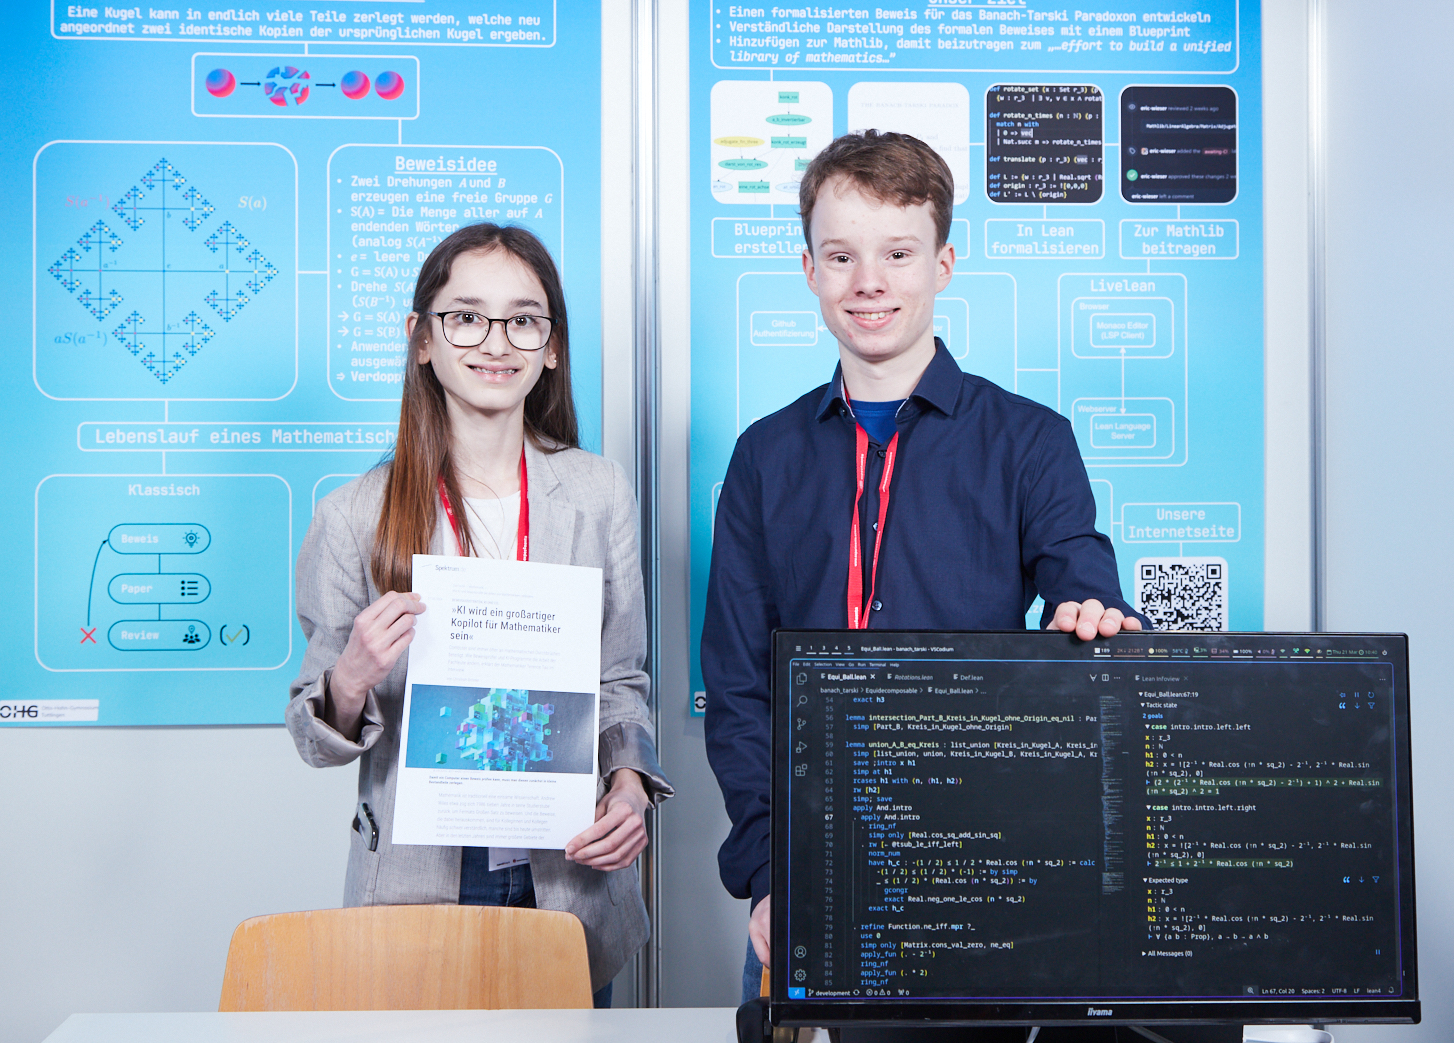
\includegraphics[scale=0.5]{M-07.jpg}

\end{figure*}
 \begin{center}

 
     \Large\textsc{Chiara Cimino, Otto-Hahn-Gymnasium Tuttlingen\\Christian Krause, Gymnasium Ochsenhausen}\\\vspace{0.7cm}

    Schülerforschungszentrum Südwürttemberg e.V.\\Standorte Tuttlingen und Ochsenhausen  \vspace{1cm}

     \today

 \end{center}~
 \clearpage
\section*{Projektübersicht}
Das Ziel unseres Jugend-forscht-Projekts des letzten Jahres war es, den Satz von Banach-Tarski, der besagt, dass wir eine Kugel allein durch Zerlegen und Neuanordnen in zwei identische Kugeln duplizieren können, mithilfe des Beweisassistenten Lean zu formalisieren und der Lean-Community zur Verfügung zu stellen. Aber warum ist diese Art der Kugelverdopplung, die ja offensichtlich den Gesetzen der Physik widerspricht, in der Mathematik überhaupt möglich? Wir machten es uns vor dem Hintergrund dieser Frage deshalb zur Aufgabe, die Problematik hinter Banach-Tarski zu beheben. Da unsere Arbeit über das Banach-Tarski-Paradoxon über die Jugend-forscht-Phase hinausging, erreichte uns in einem von zahlreichen Gesprächen mit Mathematikern der Hinweis von Fields Medaillen Träger Laurent Lafforgue, das französische Manuskript von Olivier Leroy \glqq Les intersections cachees dans le paradoxe de Banach-Tarski\grqq~in Lean zu formalisieren. Dieses Manuskript weist auf eine allgemeinere Theorie hin, in der die Problematik hinter Banach-Tarski behoben wird, weshalb wir uns intensiv mit Leroys Arbeit beschäftigten. Da diese nie in einem Journal veröffentlicht und damit auch nie offiziell geprüft wurde, begannen wir, seine Ideen mit anderen Theorien in Verbindung zu setzen und damit das Manuskript zu vervollständigen. Hierfür mussten wir zunächst einige mathematische Definitionen und Lemmata leanen, wobei es uns bereits gelang, einen Teil der Lean-Community zur Verfügung zu stellen. Ausgehend davon formalisierten wir ebenfalls einen beachtenswerten Teil von Leroys Manuskript, arbeiten aktuell an der Fertigstellung und gehen davon aus, diese zeitnah abschließen zu können. Mit Leroys Ansatz ist dann der Satz von Banach-Tarski kein Paradoxon mehr, da mit dieser Theorie die Banach-Tarski-Zerlegung nicht mehr disjunkt wäre.

test
\thispagestyle{empty}

\clearpage
\tableofcontents
\listoffigures
\thispagestyle{empty}

\begin{comment}
Kurzfassung: (bleibt hier nur vorübergehend)\\

Das Ziel unseres letztjährigen Jufo-Projekts war es, den Satz von Banach-Tarski zu leanen und der Lean-Community zur Verfügung zu stellen. Diese Arbeit ging über die Grenzen von Jufo hinaus und führte uns u.a. zu einem Kongress nach Durham, was einen Austausch mit Lean-Experten ermöglichte. Ausgehend davon erkannten wir, dass Lean noch viel mächtiger und relevanter ist, als bisher von uns angenommen wurde. Wir machten uns daher zum neuen Ziel, die mathematische Problematik hinter Banach-Tarski zu beheben. Bei einem der vielen Gespräche mit Experten erreichte uns der Hinweis von fields medal Träger Laurent Lafforgue, das Manuskript von Olivier Leroy LES INTERSECTIONS CACHEES DANS LE PARADOXE DE BANACH-TARSKI zu leanen. Das Manuskript weist auf eine allgemeinere Theorie hin, in der die Problematik hinter Banach-Tarski behoben wird. Allerdings wurde es nie in einem Journal veröffentlicht und nie offiziell geprüft. Daher gilt es für uns, das französische Manuskript zu verstehen und zu leanen.
\end{comment}
\clearpage
\setcounter{page}{1}





\section{Fachliche Kurzfassung}
Als wir letztes Jahr dabei waren, den Satz von Banach-Tarski in Lean zu formalisieren, sind wir an die Grenzen der klassischen Maßtheorie gestoßen. Der Satz von Banach-Tarski besagt nämlich, dass es theoretisch möglich ist, eine Kugel allein durch Zerschneiden und Drehen zu verdoppeln. Das ist möglich, da während des Zerschneidungsprozesses nicht messbare Teilmengen des topologischen Raums erzeugt werden. Auf der Suche nach einer Lösung für dieses Problem sind wir auf ein nie formal veröffentlichtes Manuskript von Olivier Leroy gestoßen, das verspricht das Problem der nicht messbaren Mengen von Banach-Tarski in der Theorie der Lokalen zu lösen. Dabei werden Unterlokalen anstatt von Teilmengen von topologischen Räumen verwendet. Wir haben es uns zur Aufgabe gemacht, die Grundlagen der Lokalen-Theorie und das von Leroy postulierte Maß zu verstehen und in Lean zu verifizieren. Dafür haben wir bereits viele elementare topologische Definitionen (z.B. Inklusion, Schnitt, Vereinigung und Komplement) auf die Unterlokalen übertragen und in Lean formalisiert. Ausgehend davon arbeiten wir daran, zu zeigen, dass die Caratheodory Erweiterung eines Maßes der offenen Unterlokalen auf alle Unterlokalen einige wichtige maßtheorethische Eigenschaften erfüllt. Damit ist der Satz von Banach-Tarski dann kein Paradoxon mehr, da mit dieser neuen Maßtheorie das Verdoppeln einer Kugel in zwei identische Teile nicht mehr möglich ist.


\section{Motivation und Aufgabenstellung}
\glqq Wir können eine Kugel allein durch Zerschneiden und anschließendem Drehen wieder zu zwei identischen Kopien der Ausgangskugel zusammenfügen.\grqq~Dass das mit der klassischen Mengenlehre gilt, folgt aus dem Satz von Banach-Tarski \autocite{noauthor_banach-tarski-paradoxon_2024}. Auch uns erschien diese Aussage anfänglich unglaublich, weshalb wir in unserem Jugend-forscht-Projekt des letzten Jahres den mathematischen Beweis des Banach-Tarski-Paradoxons näher beleuchteten. Indem wir den Beweis Stück für Stück durchdrangen, gingen wir automatisch den Weg einer klassischen Verifikation eines mathematischen Papers (siehe Abbildung \ref{Abb1}, linke Spalte). Da der Prozess der menschlichen Kontrolle aber durchaus fehleranfällig ist, stellten wir uns die Frage, ob man diese Fehlbarkeit nicht umgehen könnte. Dabei stießen wir auf den mathematischen Beweisassistenten Lean. Diese auf der gleichnamigen Programmiersprache Lean basierende Software erlaubt es uns, die entsprechenden mathematischen Objekte zu definieren, sowie deren Eigenschaften inkl. Beweis zu formalisieren. Ausgehend von der Typentheorie überprüft Lean die Standhaftigkeit des Beweises und markiert ggf. Fehler, was das Beweisen erleichtert. Dies bedeutet im Umkehrschluss aber auch, dass Lean den Anspruch einer absoluten mathematischen Korrektheit erheben kann (siehe Abbildung \ref{Abb1}, rechte Spalte).\\
\begin{wrapfigure}{r}{0.5\textwidth}
  \begin{center}
    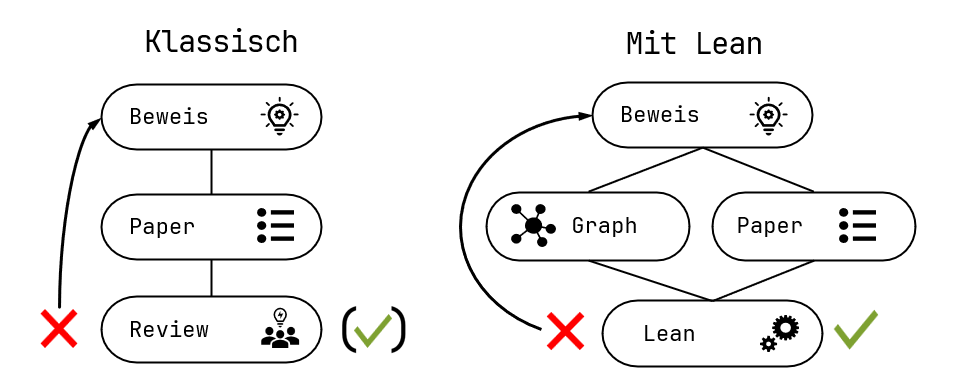
\includegraphics[width=0.48\textwidth]{Formalisierung_Grafik.png}
  \end{center}
  \caption{Verifikation mit bzw. ohne Beweisassistent}
  \label{Abb1}
\end{wrapfigure}
\noindent Bereits in Lean formalisierte mathematische Theoreme werden in einer allgemein zugänglichen Bibliothek, genannt Mathlib, gespeichert. Die Lean Community, zu der wir nun seit einem Jahr gehören, hat bereits über die Hälfte des Grundstudiums der Mathematik, sowie einige sehr fortgeschrittene Konzepte in insgesamt über eine Million Zeilen Code digitalisiert. Das ist auch der Grund, weshalb sich Mathematikerinnen und Mathematiker weltweit vernetzen, um weitere Sätze in Lean zu formalisieren.\\


\noindent Je länger wir uns jedoch mit dem Beweis des Satzes von Banach-Tarski beschäftigten, desto öfter kam die Frage auf, warum das Duplizieren einer Kugel allein durch Zerlegung der Ausgangskugel sowie anschließender Translationen und Zusammenfügen der einzelnen Teile in der Mathematik überhaupt erlaubt sein sollte, zumal dies der klassischen Physik widerspricht. Ein Ziel der Mathematik ist es, die Vorgänge um uns herum bestmöglich zu beschreiben und damit so gut wie es geht zu verstehen. Ein mathematisches Modell, das es uns erlaubt, in der Theorie Dinge zu tun, die in der Realität aber erwiesenermaßen nicht möglich sind, ist damit unvollständig. Da die Hauptaussage des Satzes von Banach-Tarski darin besteht, dass eine Kugel (insbesondere deren Volumen) verdoppelt werden kann, steht der Satz von Banach-Tarski im Gegensatz zum allgemein gültigen Erhaltungssatz in der Physik, nach dem das Gesamtvolumen nach dem Zerschneiden und Rotieren der Kugelteile zusammen wieder dem Volumen der Ausgangskugel entsprechen sollten. Da dies laut dem Satz von Banach-Tarski aber nicht der Fall ist, beschreibt das zugrundeliegende mathematische Modell des Satzes von Banach-Tarski die Realität nur unzureichend und es stellte sich uns die Frage, ob es nicht ein besseres mathematisches Modell gibt, welches genau solche Schlupflöcher nicht mehr zulässt. Um das aber sauber abgrenzen zu können, ist es essentiell, dass wir das mathematische Modell hinter dem Satz von Banach-Tarski, die klassische Maßtheorie, näher betrachten.         


\section{Kurzer Einblick in die benötigte klassische Maßtheorie (Theoretische Grundlagen)}
Die Maßtheorie \autocite{noauthor_mastheorie_2023} entstand aus dem Versuch, eine Maßfunktion zu definieren, die jeder Teilmenge eines Raumes eine sinnvolle Größe (z. B. Flächeninhalt) zuordnet. Fordert man allerdings gleichzeitig $\sigma$-Additivität und Bewegungsinvarianz dieser Maßfunktion, so muss man sich auf eine bestimmte Ansammlung von Mengen beschränken, wie Giuseppe Vitali zeigte. Diese Mengen werden als messbar bezeichnet. Auf ihnen können wir daher sog. Maße definieren:

\begin{definition}
Sei $\mathcal{A}$ eine $\sigma$-Algebra und $\mu:\mathcal{A} \to \overline{\mathbb{R}}$
eine Funktion. Man nennt $\mu$ ein Maß, falls folgende Bedingungen erfüllt sind:
\begin{itemize}
\item $\mu(\emptyset) = 0$

\item $\mu(A) \geq 0 \quad \text{für alle } A \in \mathcal{A}$

\item ($\sigma$-Additivität): Sind 
$A_1, A_2, A_3, \dotsc$ abzählbar viele paarweise disjunkte Mengen aus $\mathcal{A}$, dann gilt:
$$\mu\left(\bigcup_{k=1}^\infty A_k\right) = \sum_{k=1}^\infty \mu(A_k)$$
\end{itemize}
\end{definition}

\noindent Das wohl bekannteste Beispiel eines Maßes ist das Lebesgue-Maß \autocite{noauthor_lebesgue-mas_2023}. Es ist das Maß im euklidischen Raum, welches geometrischen Objekten ihre Länge, ihren Flächeninhalt bzw. ihr Volumen zuordnet. Die Konstruktion des Lebesgue-Maß macht es uns bspw. möglich, die Länge von offenen Intervallen zu messen. Da man nun einen Längenbegriff für offene Intervalle hat, ist es naheliegend sich zu fragen, wie es denn mit der Länge von abgeschlossenen Intervallen und anderen beliebigen Mengen aussieht. Um diesen wiederum eine sinnvolle Größe zuordnen zu können, betrachten wir die Fortsetzung des Lebesgue-Maßes auf den $\mathbb{R}^n$ mithilfe der Caratheodory-Erweiterung zu einem äußeren Maß \autocite{noauthor_auseres_2023} auf $\mathcal{P}(\mathbb{R}^n)$.\\
\noindent Unter einem äußeren Maß versteht man dabei allgemein Folgendes: 

\begin{definition}
    Sei $X$ eine Menge und $\nu:\mathcal{P}(X)\to [0;\infty]$ eine Funktion. $\nu$ heißt äußeres Maß, wenn folgende Bedingungen erfüllt sind:
\begin{itemize}
    \item $\nu(\emptyset) = 0$

\item $A \subseteq B \implies \nu(A) \leq \nu(B)~ \text{für alle}~A,B\in\mathcal{P}(X) \quad \text{(Monotonie)}$

\item $\nu\left(\bigcup_{i=1}^\infty A_i\right) \leq \sum_{i=1}^\infty \nu(A_i) \quad (\sigma\text{-Subadditivität)}$

\end{itemize}
\end{definition}
\noindent Da wir es nun mit einem äußeren Maß statt einem Maß auf der Potenzmenge von $\mathbb{R}^n$ zu tun haben, gelten Eigenschaften wie bspw. die strikte Additivität ($\mu (A\cup B)=\mu (A)+\mu(B)-\mu(A\cap B)$), welche man bei Maßen hat, nicht mehr. Die Folgen spiegeln sich unter anderem im Banach-Tarski-Paradoxon wider; eine Kugel kann ausgehend von einer komplexen Zerlegung verdoppelt werden. Um solche Kuriositäten zu umgehen, schränkt man sich üblicherweise auch beim äußeren Maß auf sog. messbare Mengen bzgl. dieses äußeren Maßes ein. Eine Menge $A$ heißt messbar bzgl. einem äußeren Maß $\mu^*$, wenn sie die Caratheodory Bedingung $\mu^*(E)=\mu^*(A\cap E)+\mu^*(A^c\cap E)$ ($E\subset X$ beliebig) erfüllt. Unserer Meinung nach ist diese Einschränkung jedoch unelegant, da wir erneut Mengen haben, denen wir keine sinnvolle Größe zuordnen können. Zu diesen Mengen gehören insbesondere auch die Banach-Tarski-Mengen. Statt die Fortsetzung eines Maßes über die klassische Mengenlehre zu betrachten und sich dann auf messbare Mengen zu beschränken, wollen wir das Problem anders lösen. Die zugrundeliegende Idee ist dabei, das äußere Maß auf der Potenzmenge der zugrundeliegenden Menge zu einem Maß zu machen. Entsprechend benötigen wir eine bessere Definition von Teilmengen, Schnitten, Vereinigungen etc.. Eine Lösung für unser Ziel bietet dabei die Theorie der Lokale.   

\begin{comment}
Dies scheitert jedoch für beliebige Teilmengen, wenn man gleichzeitig Bewegungsinvarianz und $\sigma$-Additivität fordert. Dabei versteht man unter $\sigma$-Additivität Folgendes:

\begin{definition}
    Sei $X$ eine Menge, $\mathcal{M}\subset\mathcal{P}(X)$ und $f:\mathcal{M}\to[0;\infty]$ eine Abbildung. $f$ heißt $\sigma$-additiv, wenn für endliche paarweise disjunkte $A_i\in\mathcal{M}$ mit $\bigcup_{i=1}^\infty A_i\in\mathcal{M}$ gilt:
    \[
    f\biggl(\bigcup_{i=1}^\infty A_i\bigg)=\sum_{i=1}^\infty f(A_i)
    \]
\end{definition}


\noindent 1905 zeigte aber Giuseppe Vitali, dass es im allgemeinen Fall unmöglich ist, diese Anforderungen alle gleichzeitig ohne Einschränkungen zu erfüllen. Wird die $\sigma$-Additivität bspw. auf endliche Vereinigungen beschränkt, entsteht das Inhaltsproblem von Felix Hausdorff, das ab drei Dimensionen generell unlösbar ist, mit Ausnahme der reellen Zahlen und der Ebene der reellen Zahlen.

\noindent Eine Lösung des Maßproblems wird erreicht, indem man sich auf ein eingeschränktes Mengensystem konzentriert, für das alle ursprünglichen Forderungen erfüllt werden können. Für jeden mathematischen Volumenbegriff, der ein bewegungsinvarianter Inhalt oder ein bewegungsinvariantes Maß sein soll, bedeutet dies im Umkehrschluss, dass er so eingeschränkt werden muss, dass er für bestimmte Mengen, wie die Banach-Tarski-Mengen, in die sich die Kugel zerlegen lässt, nicht definiert ist. Um nun die Mengen eines gegebenen Mengensystems messen zu können, definieret man sich eine Funktion über dieses Mengensystem wie bspw. einen Inhalt, ein Maß oder ein äußeres Maß. 

\begin{definition}

    Sei $X$ eine Menge und $\mathcal{M}\subset\mathcal{P}(X)$ mit $\emptyset\in\mathcal{M}$.
\begin{itemize}    
\item Eine Funktion $I:\mathcal{M}\to[0;\infty]$ heißt \textbf{Inhalt}, wenn $I(\emptyset)=0$ und für endliche paarweise disjunkte $A_i\in\mathcal{M}$ und $n\in\mathbb{N}$ mit $\bigcup_{i=1}^n A_i\in\mathcal{M}$ gilt die endliche Additivität: $$I\biggl(\bigcup_{i=1}^n A_i\biggl)=\sum_{i=1}^n I(A_i)$$

\item Ein $\sigma$-additiver Inhalt heißt \textbf{Maß}.

\item Eine Funktion $\nu:\mathcal{P}(X)\to[0;\infty]$ heißt \textbf{äußeres Maß}, wenn $\nu(\emptyset)=0$, die Monotonie (für $A,B\in\mathcal{M}$ mit $A\subset B$ gilt $\nu(A)\leq\nu(B)$) und die $\sigma$-Subadditivität für alle $(A_n)_{n\in\mathbb{N}}\subset\mathcal{P}(X)$: $$\nu\biggl(\bigcup_{n\in\mathbb{N}}A_n\biggl)\leq\sum_{n\in\mathbb{N}}\nu(A_n)$$

\end{itemize}
\end{definition}
Das klassische Maß, welches im $\mathbb{R}^n$ zur Volumenmessung verwendet wird, ist das sog. Lebesgue-Maß auf der Borel-$\sigma$-Algebra. Es ist das eindeutige Maß, welches $n$-dimensionalen Hyperrechtecken ihr Volumen zuordnet. Das heißt, dass das Lebesgue-Maß im Eindimensionalen einem Intervall seine Länge, im Zweidimensionalen einem Rechteck seinen Flächeninhalt und im Dreidimensionalen einem Quader sein Volumen zuordnet. Entsprechend sind die Banach-Tarski-Mengen, in die sich die Kugel zerlegen lässt, nicht Lebesgue-messbar. Es bietet sich daher an, eine Erweiterung des Lebesgue-Maßes zu betrachten, bspw. gegeben durch das äußere Maß $\lambda^*$ zum regulären Lebesgue-Maß $\lambda$, um allen Teilmengen des euklidischen Raums eine sinnvolle Größe zuordnen zu können. Das äußere Maß einer beliebigen Teilmenge $A\subseteq\mathbb{R}^n$ ist dabei gegeben durch \[
\lambda^*(A)=\inf\biggl\{\sum_{k=1}^\infty \lambda(U_k)~|~A\subseteq\bigcup_{k=1}^\infty U_k, U_k~\text{offen}\biggl\}\]
$\lambda(U_k)$ ist dabei wohldefiniert, da alle offenen Teilmengen des $\mathbb{R}^n$ Lebesgue-messbar sind. Insbesondere lässt sich für jede Lebesgue-messbare eine offene Überdeckung finden, sodass die Überdeckung und die zugrundeliegende Lebesgue-messbare Menge dasselbe Maß haben. Daher entspricht das äußere Maß einer Lebesgue-messbaren Menge dem Lebesgue-Maß dieser Menge. Wählt man nun die offene Überdeckung der Banach-Tarski-Mengen sehr \glqq sparsam\grqq, so lässt sich ihnen das äußere Maß $0$ zuordnen. Gleiches gilt für das Komplement dieser Banach-Tarski-Menge. Daher erfüllt diese die Caratheodory-Bedingung $\lambda^*(E)=\lambda^*(A\cap E)+\lambda^*(A^c\cap E)$ ($E$ ist eine beliebige Teilmenge des $\mathbb{R}^n$ und $A\subset\mathbb{R}^n$ ist Lebesgue-messbar. Es stellt sich uns daher die Frage, ob wir das zugrundeliegende System hinter dem Banach-Tarski-Paradoxon nicht so wählen können, dass die Banach-Tarski-Mengen die Caratheodory-Bedingung erfüllen. Dies würde die durch das Banach-Tarski-Paradoxon aufgezeigte Lücke in der klassischen Maßtheorie schließen und ein theoretisches Duplizieren eines Objektes nicht mehr möglich machen. Bei unseren Überlegungen stießen wir auf die sog. lokale Theorie.  
\end{comment}



\section{Die Theorie der Lokale und erste Ergebnisse unserer Arbeit}
\noindent Die Theorie der Lokale ist eine spezielle Form der punktfreien Topologie. Ein Lokal \autocite{noauthor_locale_nodate} verhält sich intuitiv wie ein topologischer Raum, der möglicherweise nicht genügend (oder sogar gar keine) Punkte besitzt. Stattdessen enthält ein Lokal offene Unterräume. Diese offenen Unterräume können so verstanden werden, dass sie eine endliche Menge an Informationen über die (hypothetischen) Punkte beinhalten. Zum Beispiel gibt es ein Lokal aller Surjektionen von den natürlichen Zahlen auf die reellen Zahlen. Dieses Lokal hat offensichtlich keine Punkte, da es keine derartigen Surjektionen gibt, sie enthält jedoch viele nichttriviale offene Teilräume.

\noindent Zu der Theorie der Lokale hat u. a.  Olivier Leroy beigetragen, z. B. durch seine Arbeit zur Maßtheorie in regulären Lokalen und deren Verbindung zum Banach-Tarski-Paradoxon (\glqq Théorie de la mesure dans les lieux réguliers\grqq~(1995) \autocite{leroy_theorie_2013}) Leroy schlägt darin vor, das Paradoxon im Rahmen der Lokale zu betrachten. 
%Ein Lokal ist dabei, intuitiv betrachtet, wie ein topologischer Raum, der möglicherweise nicht genügend Punkte hat (oder sogar überhaupt keine Punkte besitzt). Es enthält Objekte, die wir als offene Mengen bezeichnen. Allerdings ist es zulässig, dass nicht genügend Punkte vorhanden sind, um zwischen diesen offenen Mengen zu unterscheiden.
Durch die Anwendung der Theorie der Lokale zeigt er, dass es möglich ist, das Auswahlaxiom zu verwenden und dennoch sicherzustellen, dass alle \glqq Teilmengen\grqq~messbar bleiben. Dies wird durch die Einführung von Unterlokalen erreicht, die als Unterräume fungieren. In diesem Kontext ist die Fortsetzung des Lebesgue-Maßes auf die Gesamtheit der Unterlokalen von $[0;1]$ ein $\sigma$-additives Maß, welches sogar noch weitere erstaunliche gute Eigenschaften wie Reduzibilität besitzt. Dadurch werden die paradoxen Zerlegungen, wie sie bei Banach-Tarski zu finden sind und die in der klassischen Theorie zu nicht messbaren Mengen führen, in der Theorie der Lokale vermieden, da es versteckte Schnittmengen gibt, die in der klassischen Betrachtung nicht sichtbar sind.\\

\noindent Ein Punkt, den wir hier aber nicht unterschlagen dürfen, ist, dass Olivier Leroy diese Arbeit nie in einem mathematischen Fachjournal veröffentlicht hat. Stattdessen ist das Manuskript als Preprint auf offenen Repositorien wie arXiv für wissenschaftliche Arbeiten veröffentlicht worden. Im Umkehrschluss bedeutet dies, dass seine Arbeit nie peer-reviewed, d. h. durch andere Mathematiker kontrolliert, wurde. Da in seinem Manuskript außerdem mehrere Stellen sehr vage formuliert sind, haben wir es uns zur Aufgabe gemacht, seine Arbeit zunächst einmal mithilfe von Lean zu verifizieren und zu vervollständigen.

\subsection{Unser Blueprint}
Ein wesentliches Hilfsmittel, um bei bei der Arbeit in Lean die Übersicht nicht zu verlieren, ist das so genannte Lean-Blueprint-Tool \autocite{massot_patrickmassotleanblueprint_2025}, das auch in vielen großen Formalisierungsprojekten zum Einsatz kommt. 
Es bietet die Möglichkeit, alle Definitionen und Lemmata für Menschen verständlich zu formulieren und zu dem entsprechenden Lean-Code zu verlinken. Eine der wichtigsten Funktionen des Lean-Blueprint-Tools ist vermutlich der interaktive Dependency-Graph (siehe Abbildung \ref{fig:test1}). Dieser stellt alle Beziehungen zwischen den Lemmata und Definitionen übersichtlich in einem Graph dar (also welche Lemmata und Definitionen müssen zuerst fertiggestellt werden). Außerdem kann man anhand der Farbe der Knoten erkennen, wie weit die Formalisierung bereits fortgeschritten ist. \\ 
Wir haben für unser Projekt einen solchen Blueprint erstellt, der unter folgender Internetadresse veröffentlicht ist: \url{https://bergschaf.github.io/Localic-Caratheodory-Extensions/blueprint/}.\\
\begin{figure}[h]
\centering
\begin{minipage}{.5\textwidth}
  \centering
  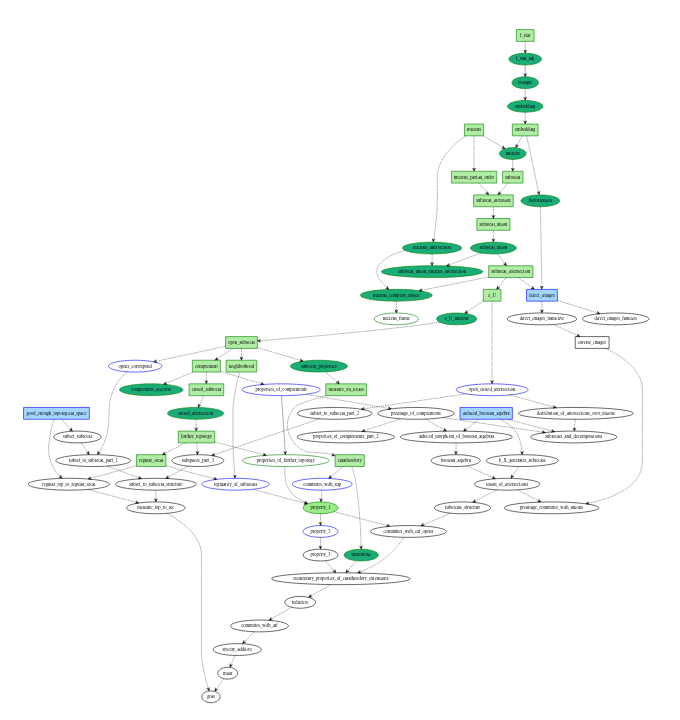
\includegraphics[width=.9\linewidth]{blueprint.png}
  \captionof{figure}{Gesamtansicht des Blueprints}
  \label{fig:test1}
\end{minipage}%
\begin{minipage}{.5\textwidth}
  \centering
  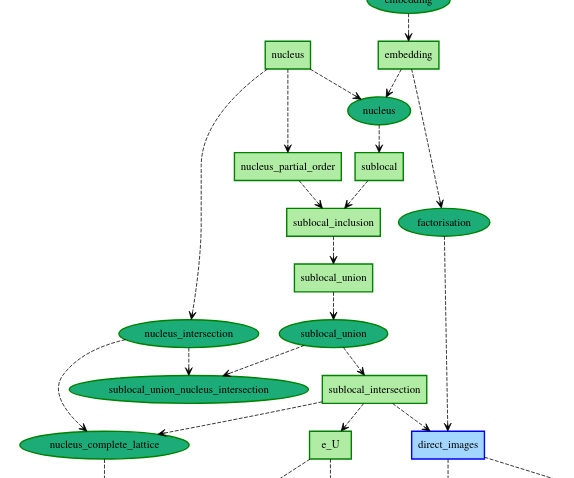
\includegraphics[width=.9\linewidth]{blueprint1.png}
  \captionof{figure}{Ein bereits formalisierter Teil des Blueprints}
  \label{fig:test2}
\end{minipage}
\end{figure}
\clearpage
\begin{itemize}
\item Im Blueprint werden Definitionen durch Rechtecke und Lemmata durch Ellipsen dargestellt.
\item Alles, was bereits fertig formalisiert ist, ist in grün dargestellt.
\item Eine Definition oder ein Lemma ist blau unterlegt, wenn alle Voraussetzungen bereits formalisiert sind und die Aussage nun bereit für die Formalisierung ist. 
\item Wenn bei einem Lemma nur der Rand eingefärbt ist, bedeutet dies, dass nur die Aussage (nicht aber der Beweis) formalisiert ist (bzw. bereit für die Formalisierung ist).
\item Ein Klick auf einen Knoten des Graphs öffnet eine Ansicht, die die entsprechende Aussage/Definition anzeigt.
\item Das Feld \textit{latex} führt zu der ausführlicheren Beschreibung der Aussage bzw. Definition im Fließtext-Teil des Blueprints.
\item Ist das Lemma oder die Definition bereits fertig formalisiert, dann gelangt man über das Feld \textit{lean} auch zu der automatisch generierten Dokumentation des dazugehörigen Lean-Codes. In dieser Dokumentation ist zu jedem Abschnitt der entsprechende Quellcode unter \textit{source} verlinkt.
\end{itemize}


\subsection{Elementare Definitionen und Lemmata der Theorie der Lokale}
Nun wollen wir aber die benötigte Theorie der Lokale besser verstehen.
Vorab definieren wir uns deshalb, was eine (partiell) geordnete Menge ist, deren Elemente wir \glqq offene Mengen von E\grqq~nennen und deren Ordnungsrelation wir mit $\subset$ schreiben. Des Weiteren klären wir nun, was man unter einem Lokal versteht.
\begin{definition}
    Ein Lokal $E$ besteht aus $(O(E),\subset)$, wobei $O(E)$ eine geordnete Menge mit Ordnungsrelation $\subset$ bezeichnet, für die folgendes gilt:
    \begin{itemize}
        \item Es existiert ein kleinstes Element $0_E$ (oder $\emptyset$) und ein größtes Element $1_E$ (oder $E$ je nach Kontext)
        \item Jede Familie $(V_i)$ von Elementen aus $O(E)$ besitzt ein Supremum (genannt Vereinigung), welche mit $\bigcup_i V_i$ bezeichnet wird.
        \item  Jedes Paar $U,V$ von Elementen aus $O(E)$ besitzt ein Infimum (genannt Schnitt von $U$ und $V$), welche mit $U\cap V$ bezeichnet wird.
        \item  Für jede Familie $(V_i)$ von Elementen aus $O(E)$ und für ein beliebiges $W\in O(E)$ gilt $W\cap\bigcup_i V_i=\bigcup_i (W\cap V_i)$
    \end{itemize}
    
\end{definition}
Wir nennen $O(E)$ auch oft die Menge an offenen Elementen von E.
\begin{example}
    Für einen Topologischen Raum $E$ bezeichne mit $O(E)$ die Menge der offenen Teilmengen von $E$. Die Ordnungsrelation ist dabei durch Inklusion gegeben.
\end{example}
Um nun mit diesen Lokalen arbeiten zu können, müssen wir definieren, was wir unter einem Morphismus zwischen zwei Lokale verstehen.
\begin{definition}
    Seien $E$ und $F$ Lokale. Ein Morphismus $f:E\to F$ wird durch eine monotone Abbildung $f^*:O(F)\to O(E)$ erzeugt, für die gilt:
    \begin{itemize}
    \item $f^*(0_F)=0_E$ und $f^*(1_F)=1_E$
    \item $f^*$ kommutiert mit endlichen Schnitten und beliebigen Vereinigungen
    \end{itemize}
\end{definition}

\begin{definition}
    Für jedes $U\in O(E)$ besitzt die Menge der $V\in O(F)$, für die gilt $f^*(V)\subset U$, also ein größtes Element, das wir mit $f_*(U)$ bezeichnen werden.
\end{definition}

\begin{lemma}
    Für jeden Morphismus von Lokalen $f:E\to F$ sind die folgenden Eigenschaften äquivalent:
    \begin{itemize}
\item $f^*$ ist surjektiv  
\item  $f_*$ ist injektiv  
\item $f^* f_*=1_{O(E)}$ 
\end{itemize}
Man nennt einen Morphismus von Lokalen, der diese Eigenschaften erfüllt, Einbettung.
\end{lemma}
Eine weitere zentrale Abbildung ist der Nukleus, welchen wir im Folgenden definieren:

\begin{definition}\label{def:nukleus}
    Ein Nukleus \autocite[S. 485]{mac_lane_sheaves_1994} ist eine Abbildung $e:O(E)\to O(E)$ mit den folgenden drei Eigenschaften:
    \begin{itemize}
        \item $e$ ist idempotent, d. h. $e\circ e=e$
        \item $U\leq e(U)$ für alle $U\in O(E)$
        \item $e(U\cap V)=e(U)\cap e(V)$ für alle $U,V\in O(E)$
    \end{itemize}
\end{definition}


\begin{lemma}\label{lemma1}
\autocite[S. 484]{mac_lane_sheaves_1994} Sei $E$ ein Lokal und $e:O(E)\to O(E)$ eine monotone Abbildung. Die folgenden Aussagen sind äquivalent:
\begin{itemize}
\item Es existiert ein Lokal $X$ und ein Morphismus $f:X\to E$ mit $e = f_∗f^∗$.
\item $e$ ist idempotent mit einer Einbettung
\item $e$ ist idempotent für alle $U,V\in O(E), e(U)\supset U$ und $e(U\cap V)=e(U)\cap e(V)$ (Also $e$ ist ein Nukleus)
\end{itemize}
 \end{lemma}

\begin{lemma}
    Sei  $i:X\to E$ eine Einbettung und $f:Y\to E$ ein Morphismus von Lokalen. Damit sich  $f$ durch $i$ faktorisieren lässt, ist es notwendig und hinreichend, dass für jedes $V\in O(E)$ gilt: $i^* i_* (V)\subset f^* f_* (V)$.
\end{lemma}

\subsection{Unterlokale}
Ein wesentliches Konzept, das wir in unserer Arbeit benötigen, ist das Konzept der Unterlokale, weshalb wir diese nun im Folgenden näher betrachten wollen.
\begin{definition}
    Ein Unterlokal $X$ eines Lokals $E$ wird durch eine Abbildung $e_X:O(E)\to O(E)$ definiert, die die Eigenschaften eines Nukleus erfüllt (Definition \ref{def:nukleus},Lemma \ref{lemma1}). Folglich ist das von $X$ erzeugte Lokal gegeben durch $O(X)=Im(e_X)=\{V\in O(E) | e_X(V)=V\}$ und die zugehörige Einbettung $i_X:X\to E$ ist durch $i^∗_X(V)=e_X(V)$, $(i_X)_∗(U)=U$ definiert. \autocite{noauthor_sublocale_nodate}
\end{definition}


Um mit diesen Unterlokalen arbeiten zu können, definieren wir nun die Inklusion, Vereinigung und den Schnitt von Unterlokalen. Später werden wir zeigen, dass die Menge aller Nuklei $N(A)$ auf einem Lokal $A$ einen Frame \autocite{noauthor_frame_nodate} bilden. \\

% Ich finde des mit der Dualen Ordnung irgendwie elegant, ist halt die Frage wie viel uns das bringt...
Mit der Ordnungsrelation $X \le Y \iff X h \le Y h$ für alle $h$, und alle Nuklei $X$ und $Y$ bilden die Nuklei eine Halbordnung. Die Ordnung der Unterlokale ist Dual zu dieser Ordnung definiert: 

% TODO quelle auch von berühmten leuten ((StoneSpaces S. grob 50, 2.5)) da gibs bessere
\begin{definition}
    Die Inklusion zweier Unterlokale $X$ und $Y$ von $E$ lässt sich damit folgendermaßen definieren:
    $$X \subseteq Y \iff e_X(h) \supseteq e_Y(h)$$
    für all $h \in E$
\end{definition}
% Sollen wir hier bei \subseteq bleiben oder \le verwenden??



Die Unterlokale bilden daher eine Duale Ordnung zu den Nuklei. \autocite[S. 51]{johnstone_stone_1982} \autocite{noauthor_categorydual_nodate}% TODO QUelle https://proofwiki.org/wiki/Category:Dual_Orderings
Dadurch können Resultate auf der einen Ordnung zu der dualen Version auf der anderen Ordnung übertragen werden. Es ist beispielsweise bekannt, dass eine Ordnung genau dann einen Verband (engl: Lattice) bildet, wenn die duale Ordnung ebenfalls einen Verband \autocite{noauthor_verband_2024} bildet \autocite{noauthor_dual_nodate}. % Quelle Verband : https://de.wikipedia.org/wiki/Verband_(Mathematik) % QUelle dual lattice https://proofwiki.org/wiki/Dual_of_Lattice_Ordering_is_Lattice_Ordering
In unserem Fall reicht es daher aus, zu zeigen, dass die Nuklei (bzw. die Unterlokale) einen Verband bilden, um von der selben Struktur auf den Unterlokalen (bzw. den Nuklei) zu wissen. \\
Wir können diese Definition der Inklusion nun verwenden, um zwei besondere Nuklei genauer zu betrachten:
\begin{definition}
    Wir bezeichnen den folgenden Nukleus mit: $\top_n (a) = \top_E$. $\top_E$ symbolisiert das größte Element von $E$. Wir wissen, dass es existiert, da $E$ einen Frame bildet.
\end{definition}
Man sieht, dass $\top_n$ der größte Nukleus ist, da er im punktweisen Vergleich, alle anderen Nuklei enthält.
\begin{definition}
    $\bot_n$ bezeichnet folgenden Nukleus: $\bot_n (a) = a$
\end{definition}
Dieser Nukleus ist \glqq kleiner \grqq{} als alle anderen Nuklei, da jeder Nukleus $x$ die Bedingung $a \le x(a)$ erfüllen muss. Da die Unterlokale eine duale Ordnung zu den Nuklei bilden, wissen wir, dass der größte Nukleus dem kleinsten Unterlokal entspricht. Der kleinste Nukleus gehört daher zur größten Unterlokale:
$$\top_s = \bot_n \text{ und } \bot_s = \top_n$$
$\top_s$ bezeichnet im Folgenden also das größte und $\bot_s$ das kleinste Unterlokal. \\

Da es deutlich mehr Unterlokalen einer Lokale als Teilmengen des entsprechenden Topologischen Raums gibt, können wir den Schnitt und die Vereinigung von Unterlokalen nicht punktweise definieren.

Peter Johnstone definiert daher  in seinem Buch \glqq Stone spaces\grqq{} \autocite{johnstone_stone_1982} das beliebige infimum der Nuklei folgendermaßen: \\
\begin{definition}
    Der Schnitt einer Menge $S$ an Nuklei auf $E$ bildet einen Nukleus mit folgender Funktion:
    $$(\bigcap_n S)(a) = \bigcap \{j(a) | j \in S\} $$ für alle $a \in E$\\
    
\end{definition}
Um zwischen dem Schnitt von Nuklei und Unterlokalen zu unterscheiden, bezeichnet $\bigcap_n$ den Schnitt von Nuklei und $\bigcap_s$ den Schnitt von Unterlokalen. \\
Wir haben analog zu Johnstone in Lean verifiziert, dass die Funktion $\bigcap_n S(a)$ die drei Bedingungen für einen Nukleus erfüllt. % TODO lean link
Außerdem haben wir verifiziert, dass dieser Nukleus auch die Bedingungen eines beliebigen Infimums erfüllt \autocite{noauthor_mathlibordercompletelattice_nodate}.\\ 
Dieses Infimum der Nuklei bildet aufgrund der Dualen Ordnung ein Supremum der Unterlokalen \autocite{noauthor_supremum_nodate}. Leroy hat aber ebenfalls ein Supremum auf den Unterlokalen definiert:
\begin{definition}
    Der Schnitt einer Menge $S$ an Unterlokalen von $E$ bildet einen Nukleus mit folgender Funktion:
    $$(\bigcup_s S)(a) = \bigcup \{w \in E | \forall x \in S,w \subseteq x\} $$ für all $a \in E$
\end{definition}
% TODO Quelle leroy seite 5
Hier haben wir ebenfalls bereits in Lean verifiziert, dass die Funktion die Bedingungen für einen Nukleus und die Bedingungen des beliebigen Supremums erfüllt. \\

\begin{lemma}
    Die Definitionen von Johnstone und Leroy \autocite[S. 5]{leroy_theorie_2013} sind äquivalent: 
        $$(\bigcap_n S) (a) = (\bigcup_s S) (a)$$ für alle Mengen an Nuklei $S$ und für alle $a \in E$ \\
        %TODO hier müsste man eig definieren wie man Unterlokale zu Nuklei konvertiert und umgekehrt
\end{lemma}
\begin{proof}
    Da wir verifiziert haben, dass beide Suprema die Bedingungen für beliebige Suprema erfüllen, wissen wir, dass beide eine obere Schranke für $S$ bilden \autocite{noauthor_beschrankte_2021}. 
    Wir wissen aber ebenfalls, dass beide Suprema die kleinste obere Schranke bilden, daher haben wir $(\bigcap_n S) \le (\bigcup_s S)$ und  $(\bigcup_s S) \le (\bigcap_n S)$, woraus die Gleichheit folgt.
    % TODO lean link
\end{proof}



Infima von Unterlokalen (bzw. Suprema von Nuklei) lassen sich schwerer mit einer expliziten Formel beschreiben \autocite[S. 6]{leroy_theorie_2013}, es kann aber auch das Supremum aller unteren Schranken verwendet werden.\\
% Definition Infimum
\begin{definition}
    Das Infimum einer Menge $S$ an Unterlokalen von $E$ entspricht dem Supremum der unteren Schranke von $S$.
    $$\bigcap_s S = \bigcup_s \{w \in E | w \le x\}$$ für alle $x \in S$
\end{definition}

\subsection{Offene und abgeschlossene Unterlokale}
Die offenen Mengen eines Topologischen Raums bilden immer eine Lokale. Die Elemente dieser Lokale hängen exakt mit den offenen Unterlokalen zusammen, die daher also den offenen Mengen eines Topologischen Raums entsprechen. Die Komplemente dieser offenen Unterlokalen (bzw. offenen Mengen) bilden die abgeschlossenen Unterlokalen, die mit den abgeschlossenen Mengen eines Topologischen Raums zusammenhängen.\\
Johnstone \autocite[S. 50]{johnstone_stone_1982} und MacLane \autocite[S. 488]{mac_lane_sheaves_1994} definieren beide in ihren Büchern die offenen Unterlokalen folgendermaßen:
\begin{definition}
\label{def:open}
    Jedes Element $v$ einer Lokale $E$ erzeugt eine offene Unterlokale von $E$ mit der Funktion:
    $$o_v(a) = v \Rightarrow a$$ für alle $a \in E$. % ($\implies$ symbolisiert die Heyting Implikation)% TODO quelle heyting implication
\end{definition}
Johnstone und MacLane verwenden hier $v \Rightarrow a$, die sogenannte Heyting-Implikation (auch relatives-Pseudokomplement) \autocite{noauthor_heyting-algebra_2024}\autocite{noauthor_heyting_nodate}.
\begin{definition}
    Die Heyting-Implikation erfüllt die Bedingung $a \le b \Rightarrow c$ genau dann, wenn $a \cap b \le c$ für alle $a$, $b$ und $c$. Eine Heyting Algebra ist ein Verband, bei dem diese Operation für alle Elemente definiert ist.
\end{definition}
Die Heyting-Implikation kann hier verwendet werden, da die Elemente einer Lokale eine vollständige Heyting Algebra bilden.\\
% TODO Quelle Open Sublocals (Mclane488) (Stonespaces S.50) (Leroy)
Anhand dieser Eigenschaften haben wir hier auch in Lean wieder verifiziert, dass es sich bei $o_v$ für alle $v \in E$ um einen Nukleus handelt \autocite{noauthor_leroyopen_sublocales_nodate}. % TODO lean link. 

\begin{lemma}
    \label{lem:himp_eq}
    Die Definition der offenen Unterlokale von Johnstone \ref{def:open} ist äquivalent zu der Definition von Leroy: 
$$o_v(a) = \bigcup \{ W \in E | W \cap V \le a \}$$
\end{lemma}
\begin{proof}
Es genügt hier zu zeigen, dass $v \Rightarrow a$ das größte Element in der Menge $S = \{ W \in E | W \cap V \le a \}$ ist. 
Wir wissen, dass $c \le c \Rightarrow a$ genau dann, wenn $f c \cap v \le a$, daher sind alle Elemente $S$ kleiner oder gleich wie $v \Rightarrow a$.
\end{proof}
Wir können nun anhand einiger Eigenschaften der offenen Unterlokalen (analog zu Leroy \autocite[S. 10]{leroy_theorie_2013}) zeigen, dass die offenen Unterlokalen von $E$ nahezu austauschbar mit ihrem entsprechenden Element von $E$ verwendbar sind. Um den folgenden Teil etwas übersichtlicher darzustellen, verwenden wir die Notation $[V]$ für $o_v$. \\
Uns ist es gelungen, zu verifizieren, dass $[V] \subseteq [U]$ genau dann, wenn $V \subseteq U$ für alle $u, v \in E$. %TODO Blueprint Link.
Wir haben außerdem gezeigt, dass die offenen Unterlokalen mit beliebigen Suprema kommutieren: 
$$\bigcup_i [V_i] = [\bigcup_i V_i]$$ %TODO Blueprint link
Für alle Familien $V_i$ aus Elementen von $E$. \\
Die offenen Unterlokalen kommutieren zudem mit endlichen Infima: 
$$[U \cap V] = [U] \cap [V]$$ %% TODO Blueprint link
für alle $U, V \in E$. Da wir diese Eigenschaften (neben einigen anderen) auch in Lean formalisiert haben, sind sie auch im \href{https://bergschaf.github.io/Localic-Caratheodory-Extensions/blueprint/sect0004.html#def:open_sublocal}{Blueprint} zu finden. \\
Johnstone, MacLane und Leroy definieren die abgeschlossenen Unterlokalen alle ähnlich: 
% Definition Closed Sublocals (Mclane 488) (Stonespaces S.50)

\begin{definition}
    Jedes Element $V \in E$ erzeugt eine geschlossene Unterlokale mit dem Nukleus: 
    $$c_v(a) = v \cap a$$
    für alle a.
\end{definition}
%TODO quelle
Es lässt sich leicht verifizieren, dass es sich bei $c_v$ um einen Nukleus handelt. Leroy behauptet außerdem, dass es sich bei $c_v$ für alle $v \in E$ um das Komplement von $o_v$ handelt. Dies lässt sich anhand der folgenden Eigenschaften zeigen:
\begin{lemma}
    $$c_v \cap o_v = \bot_s \text{  und  } c_v \cup o_v = \top_s$$
    für alle $v \in E$. 
\end{lemma}
Wir können also definieren:
\begin{definition}
    Das Komplement einer offenen Unterlokale $o_v$ entspricht $o_v^c = c_v$ für alle $v \in E$
\end{definition}
\begin{definition}
    Im Folgenden bezeichnen $O(E)$ und $C(E)$ die Menge der offenen bzw. abgeschlossenen Unterlokalen von $E$
\end{definition}
Mit diesen Definitionen der offenen und geschlossenen Unterlokalen können wir nun einige klassische topologische Operationen auf den Unterlokalen definieren. Diese werden später oft in verschiedenen Beweisen verwendet.
\begin{definition}
    Der Abschluss einer Unterlokalen $X$ entspricht der kleinsten geschlossenen Unterlokalen, die $X$ enthält:
        $$\overline{X} = \bigcap \{W \in C(E) \mid X \le W \}$$
\end{definition}
\begin{definition}
    Das Äußere einer Unterlokalen $X$ entspricht der größten offenen Unterlokalen, die disjunkt zu $X$ ist: $$Ext~X = \bigcap \{W \in O(E) \mid W \cap X = \bot_s \}$$
\end{definition}

\begin{definition}
    Die offene Umgebung eines Unterlokals $X$ ist die Menge aller offenen Unterlokalen $V$, für die gilt $X \subseteq V$
\end{definition}

\begin{definition}
    Ein Lokal $E$ heißt regulär, wenn für alle offenen Unterlokale $U$ von $E$ die offenen Unterlokale $V$ von $E$ mit $\overline{V} \subseteq U$ ganz $U$ abdecken.
\end{definition}
Sei $E$ im Folgenden ein reguläres Lokal.
\begin{lemma}
\label{lem:regular_sublocal}
    In einem regulären Lokal entspricht jedes Unterlokal $U$ dem Schnitt der offenen Umgebung von $U$.
\end{lemma}
Jetzt haben wir die notwendigen Voraussetzungen definiert und kleinere Lücken geschlossen, um mit der Maßtheorie über Lokalen zu beginnen.


\section{Maßtheorie über Lokale und weitere Ergebnisse unserer Arbeit}\label{Maßtheorie über Lokale}
%Analog zum Aufbau aus dem Blueprint 
Die Maßtheorie über Lokale bietet einen abstrakten Zugang zur Definition von Maßen, der direkt auf der Struktur offener Mengen bzw. offener Unterlokale basiert, ohne auf Punkte oder klassische Mengenoperationen angewiesen zu sein. Statt einzelner Punkte stehen hier offene Teilstrukturen und deren algebraische Beziehungen im Mittelpunkt. Dieser Ansatz erlaubt es, Maßbegriffe auf einer rein strukturellen Ebene zu formulieren. Entsprechend definieren wir ein Maß über Lokale wie folgt:

\begin{definition}
Ein Maß auf einem Lokal $E$ ist eine Abbildung $\mu:O(E)\to \mathbb{R}^{+}$, die für alle Unterlokale $U$ und $V$ von $E$ die folgenden Eigenschaften erfüllt:  
\begin{itemize}
\item $\mu(\emptyset)=0$  
\item $U\subseteq V\implies\mu(U)\leq\mu(V) $ 
\item $\mu(U\cup V)=\mu(U)+\mu(V)-\mu(U\cap V)$  
\item $\mu\left(\bigcup_i V_i\right)=\sup_i\mu(V_i)$ für jede monoton steigende Familie $(V_i)_{i\in\mathbb{N}}$ von Elementen aus $O(E)$. D. h., dass für alle $i,j\in\mathbb{N}$ ein $k\in\mathbb{N}$ gibt mit $V_i\cup V_j\subset V_k$ bzw. $V_i\subset V_k$ und $V_j\subset V_k$.
\end{itemize}

\end{definition}
Analog zu der klassischen Maßtheorie, können wir auch hier eine Erweiterung eines Maßes definieren.

\begin{definition}
Sei $E$ ein Lokal und $\mu$ ein Maß über $E$. Sei $A$ ein beliebiges Unterlokal von $E$, also insbesondere nicht unbedingt offen. Dann ist $\mu (A)$ definiert durch $\mu (A):=\inf\{\mu (U)~|~A\subset U, U\in O(E)\}$.
\end{definition}


\subsection{Elementare Eigenschaften der Maßtheorie über Lokale}
Wir sind dabei, in Lean zu zeigen, dass ein Maß über Lokale die Eigenschaften eines klassischen Maßes erfüllt, die da wären:
\begin{lemma}
Für jedes Maß $\mu$ mit Caratheodory-Erweiterung über ein Lokal $E$ werden folgende Eigenschaften erfüllt:
\begin{itemize}
    \item Für alle Unterlokale $A,B$ von $E$ gilt $A\subseteq B\Rightarrow\mu(A)\leq\mu(B)$ (\textbf{Monotonie})
    \item Für offene Unterlokale $U$ von $E$ gilt $\mu(U)+\mu(E\setminus U)=\mu(E)$
    \item Für offene Unterlokale $U$ von $E$ und Unterlokale $A$ von $E$ gilt $\mu(A)=\mu(A\cap U)+\mu(A\cap(E\setminus U))$
     \item Für eine monoton steigende Familie $(V_i)_{i\in\mathbb{N}}$ von offenen Unterlokalen von $E$ gilt: $\mu(\sup_i V_i)=\sup_i\mu(V_i)$
    \item Für eine monoton steigende Familie $(V_i)_{i\in\mathbb{N}}$ von offenen Unterlokalen von $E$ und für ein Unterlokal $A$ von $E$ gilt: $\mu(A\cap\sup_i V_i)=\sup_i\mu(A\cap V_i)$
    \item Für eine monoton fallende Familie $(V_i)_{i\in\mathbb{N}}$ von offenen Unterlokalen von $E$ gilt $\mu(\inf_i V_i)=\inf_i\mu(V_i)$
\end{itemize}
Insbesondere gilt für zwei offene Unterlokale $U, V$ von $E$ und einem Unterlokal $A$ von $E$
\[
\mu(A\cap(U\cup V))=\mu(A\cap U)+\mu(A\cap V)-\mu(A\cap U\cap V)
\]
\end{lemma}
\noindent Dass wir die grundlegenden Bausteine der klassischen Maßtheorie übertragen können, hat zur Folge, dass auch andere fundamentale Konzepte in der Theorie der Lokale erhalten bleiben. Insbesondere wird es uns dadurch erleichtert, die Theorie der Lokale zu verstehen und bestehendes Wissen aus der klassischen Maßtheorie entsprechend anzupassen.\\
Um exemplarisch den Prozess des Beweisens einer solchen Eigenschaft zu zeigen, beschäftigen wir uns nun mit der folgenden Eigenschaft. Den Beweis dafür haben wir dabei eigenständig ausgearbeitet.
\begin{lemma}
    Für alle offenen Unterlokalen $U$ von $E$ gilt: 
    $$\mu(U) + \mu(U^c) = \mu(\top_s)$$ % TODO ggf das umformulieren oder die anderen eigenschaften in der Notation anpassen
\end{lemma}
\begin{proof}
% TODO leroy quelle
    Sei $V$ die Familie der offenen Umgebungen von $U^c$. Sei $W$ die Familie der äußeren von $V$: $W_i := Ext(V_i)$ für alle $i$. Die Vereinigung von $W$ entspricht $U$, da $\bigcap_i V_i = U$ (siehe Lemma \ref{lem:regular_sublocal}). $W$ ist außerdem monoton filtriert, da $U \cup V$ für alle $U, V \in W$ ein Element bildet, das $U$ und $V$ enthält. $U \cup V$ ist in $W$ enthalten, da endliche Schnitte von offenen Umgebungen auch immer eine offene Umgebung bilden. Da $V$ also unter endlichen Schnitten abgeschlossen ist, sind die äußeren von $V$ (also $W$) unter endlichen Vereinigungen abgeschlossen. Da $W$ also monoton filtriert ist, können wir (aufgrund der Eigenschaften von $\mu$ auf den offenen Unterlokalen) folgende Umformung durchführen: $$\mu(U) = \mu(\bigcup_i W_i) = \sup_i \mu (W_i)$$
    Des Weiteren zeigen wir, dass $\mu(W_i) + \mu(V_i) \le \mu(\top_s)$ für alle $i$. Aufgrund der Definition des äußeren wissen wir, dass $W_i \cap V_i = \bot_s$ und $W_i \cup V_i \le \top_s$. Da $\mu(\bot_s) = 0$ und da $\mu$ monoton ist, können wir zeigen: 
    $$\mu(W_i) + \mu(V_i) = \mu(W_i) + \mu(V_i) + \mu(W_i \cap V_i) = \mu(W_i \cup V_i) \le \mu(\top_s)$$ für alle $i$. 
    Da $U^c \le V_i$ (also $\mu(U^c) \le \mu (V_i)$) wissen wir: $\mu(W_i) + \mu(U^c) \le \mu(\top_s)$. Da dies für alle $i$ gilt und wir vorher gezeigt haben, dass $\mu(U) = \sup_i \mu (W_i)$, haben wir die eine Richtung gezeigt: $\mu(U) + \mu(U^c) \le \mu(\top_s)$. \\
    Um die andere Richtung der Inklusion zu zeigen, beginnen wir mit der Definition der Caratheodory Erweiterung: $\mu(U^c) = \inf_i \mu(V_i)$. Daher wissen wir, dass $\mu(U^c) + \epsilon > \inf_i \mu(V_i)$ für alle $\epsilon > 0$. Es gibt also für alle $\epsilon > 0$ ein $W \in V_i$, sodass $\mu(U^c) + \epsilon > \mu(w)$. Da $W$ eine offene Umgebung von $U^c$ ist, haben wir: $W \cup U^c \ge \top_s$ und daher: $\mu(W) \cup \mu(U) \ge \mu(\top_s)$. Daraus folgt: $$\mu(\top_s) \le \mu(U) + \mu(U^c) + \mu(\epsilon)$$ Da dies für alle $\epsilon > 0$ gilt, können wir $\mu(\epsilon)$ auch mit $inf \{ \mu(\epsilon) | \epsilon > 0\} = 0$ ersetzen und können damit den Beweis abschließen.
\end{proof}
Unsere (nicht verkürzte) Lean Formalisierung dieses Beweises nimmt ungefähr 200 Code-Zeilen ein \autocite{noauthor_leroy_lemme3_nodate}. Am Vergleich zu den vier Zeilen im Originaldokument von Leroy \autocite[S. 25]{leroy_theorie_2013} erkennt man gut, dass es, vor allem in diesem Fall, oft ein signifikanter Aufwand ist, schriftliche Beweise in Lean zu formalisieren. Es ist nämlich nicht nur nötig, den Text in Code zu übersetzen, sondern es müssen oft auch wichtige Teile des Beweises \glqq neu gefunden\grqq{} werden, da sie im Originaldokument nicht enthalten sind.

\subsection{Neue Eigenschaften der Maßtheorie über Lokale}
Um den Banach-Tarski-Mengen eine sinnvolle Größe in der Theorie der Lokale zuordnen zu können, braucht es selbstverständlich mehr als nur die auch in klassischen Maßen auffindbaren elementaren Eigenschaften. Aktuell sind wir dabei in Lean zu zeigen, dass ein Maß über Lokale mit Caratheodory-Erweiterung folgende neue Eigenschaften aufweist: 
\begin{lemma}
Sei $E$ ein Lokal und $\mu$ ein Maß über $E$ mit Caratheodory-Erweiterung. Dann besitzt $\mu$ folgende Eigenschaften:
\begin{itemize}
    \item Für alle Unterlokale $A, B$ von $E$ gilt $\mu (A\cup B)=\mu (A)+\mu(B)-\mu(A\cap B)$ (\textbf{strikte Additivität})
    \item Für eine Familie $(A_i)_{i\in\mathbb{N}}$ von Unterlokalen von $E$ gilt $\mu (\inf A_i)=\inf\mu (A_i)$ (\textbf{kommutiert mit Infimumbilden}) 
    \item Sei $A$ ein Unterlokal von $E$. Die Menge $\{A'\subset A~\text{Unterlokal von}~E~|~\mu(A')=\mu(A)\}$ hat ein minimales Element (\textbf{Reduzierbarkeit}). 
\end{itemize}
\end{lemma}

\noindent Insbesondere gilt nun die strikte Additivität des Maßes mit Caratheodory-Erweiterung für alle Unterlokale eines gegebenen Lokals. Da jede Teilmenge einer gegebenen Menge ein Unterlokal induziert, lässt sich die strikte Additivität auf diese Teilmengen übertragen. Entsprechend können wir festhalten, dass die Caratheodory-Erweiterung nun bessere Eigenschaften hat, die es zusammen mit der besseren Definition des Schnitts möglich machen, den Banach-Tarski-Mengen eine sinnvolle Größe zuzuordnen und dem \glqq Banach-Tarski-Paradoxon\grqq~seinen paradoxen Charakter entziehen, indem ein Duplizieren einer Kugel im Sinne des Satzes von Banach-Tarski nicht mehr möglich ist.


\section{Einbettung in Topostheorie (ein Ausblick)}
Die von Alexander Grothendieck in den 1960er Jahren aufgestellte Topostheorie ist ein Teilgebiet der Mathematik, das Kategorien, Logik und Geometrie verbindet. 

Ein Topos ist dabei durch seine Struktur definiert: Er besitzt exponentielle Objekte (Verallgemeinerung von Funktionsräumen), alle endlichen Limiten und Kolimiten, sowie einen Subobjektklassifikator, der logische Aussagen beschreibt. Diese Eigenschaften ermöglichen die Entwicklung einer internen Logik, die klassisch oder intuitionistisch sein kann. Beispiele umfassen die Kategorie der Mengen und die Kategorien von Garben. Wie wir im Folgenden sehen werden, können wir Lokale kategorientechnisch über Topoi, genauer gesagt Grothendieck-Topoi beschreiben. 

\begin{proposition}
Für einen Grothendieck-Topos $\mathcal{E}$ sind die folgenden Aussagen äquivalent:  
\begin{itemize}
\item $ \mathcal{E} $ ist lokal, d. h. $ \mathcal{E} $ ist äquivalent zur Garbenkategorie $\text{Sh}(X)$ auf einer Lokale $X$
\item $ \mathcal{E} $ wird durch die Unterobjekte seines terminalen Objekts $ 1 $ erzeugt.  
\end{itemize}
\end{proposition}

\begin{proposition}
Jede Einbettung $I: \mathcal{E} \to \text{Sh}(X) $ eines Topos in einen lokalen Topos erzwingt, dass der Ausgangstopos $ \mathcal{E} $ ebenfalls lokal ist.
\end{proposition}

Damit besitzen lokale Topoi eine intrinsische Struktur, die nicht verloren geht, wenn andere Topoi in sie eingebettet werden.
\begin{proposition}
    Sei $ I: X \to Y $ eine Abbildung von Lokalen und $ I: \text{Sh}(X) \to \text{Sh}(Y) $ der entsprechende geometrische Morphismus.  
\begin{itemize}

\item Die Abbildung $ I: X \to Y $ ist genau dann eine Surjektion von Lokalen, wenn $ I: \text{Sh}(X) \to \text{Sh}(Y) $ eine Surjektion von Topoi ist.  

\item Die Abbildung $ I: X \to Y$ ist genau dann eine Einbettung von Lokalen, wenn $ I: \text{Sh}(X) \to \text{Sh}(Y) $ eine Einbettung von Topoi ist. 
\end{itemize}
\end{proposition}

Aus diesen Äquivalenzen lässt sich folgern, dass die kategorialen Eigenschaften geometrischer Morphismen eine direkte Entsprechung in der lokalen Struktur der ursprünglichen Lokale haben.

\begin{proposition}\label{prop24}
    Für jedes Lokal $ X $ entsprechen die Unterlokale von $ X $ genau den Untertopoi von $ \text{Sh}(X) $; oder äquivalent dazu entsprechen die Kerne (Nuklei) auf dem Frame $ \mathcal{O}(X) $ genau den Lawvere-Tierney-Topologien im Topos $ \text{Sh}(X) $.
\end{proposition}

Hiermit wird deutlich, dass jede Teilstruktur eines Lokals, wie sie durch Unterlokale beschrieben wird, auf die Teilstrukturen des zugehörigen Topos übertragen werden kann. Dasselbe gilt für die Nuklei auf $\mathcal{O}(X)$, welche den durch Lawvere-Tierney-Topologien beschriebenen kategorialen Eigenschaften entsprechen.

Anhand dessen wird deutlich, dass wir die bisherige Arbeit über Lokale analog auf Topoi übertragen können. Diese formelle Übertragung der Maßtheorie über Lokale in die allgemeinere Welt der Topoi mithilfe von Lean ist ebenfalls Ziel dieser Jugend-forscht-Arbeit. Hierfür müssen wir aber zunächst die Grundgedanken der Maßtheorie über Lokale in Lean formalisieren, weshalb wir uns zuerst auf das Formalisieren des Manuskripts von Olivier Leroy konzentrieren.   

\section{Zusammenfassung der Ergebnisse und kritische Betrachtung}
Ein wichtiger Teil unseres Projektes ist es, die Resultate nicht nur zu verstehen und zu Papier zu bringen, sondern parallel auch in Lean zu formalisieren. Das hat einerseits natürlich den Vorteil, dass Beweise mit Lean automatisch sicher verifiziert werden können. Ein weiterer wichtiger Aspekt, bei dem Lean großes Potenzial hat, ist die Zusammenarbeit zwischen Mathematikern. Hier spielt natürlich auch wieder die Verifizierung eine Rolle, da so vor allem in großen Teams nicht jedes Mitglied alle Beweise verstehen und überprüfen muss. Für unser Projekt war es allerdings von deutlich größerer Bedeutung, dass Lean dem Nutzer die Möglichkeit gibt, Definitionen mit einer formalen Sprache standardisiert zu verfassen und in der Mathlib \autocite{noauthor_leanprover-communitymathlib4_2025} 
zu veröffentlichen. Bei dem Aufnahmeprozess in die Mathlib werden Definitionen zudem ausführlich mit anderen Mitwirkenden der Mathlib diskutiert, was die Möglichkeit für wertvolles Feedback gibt. Da eine sogenannte \glqq Pull Request\grqq{} \autocite{noauthor_how_nodate}
dadurch (in Abhängigkeit von der Komplexität des hinzugefügten Materials) auch etwas länger dauern kann, haben wir uns vorgenommen, bereits vor dem Ende unseres Projektes erste Definitionen und Resultate in der Mathlib zu veröffentlichen. \\
Ein Beispiel für eine Pull Request, die bereits zur Mathlib hinzugefügt wurde \autocite{noauthor_github_nodate} ist das Lemma, das ein beliebiges Infimum auf einer Ordnung einen beliebigen Supremum auf der Dualen Ordnung entspricht (bzw. ein beliebiges Supremum entspricht einem beliebigen Infimum auf der Dualen Ordnung). \\ %(TO DO link zu github mathlib code vlt...) 
Ein weiteres Resultat, das bereits von zwei Reviewern kontrolliert wurde, ist eine verallgemeinerte Version von Lemma \ref{lem:himp_eq}, die besagt, dass die Heyting Implikation auch als Supremum ausgedrückt werden kann. Unsere Version in der Mathlib enthält dazu noch einige allgemeine Hilfslemmata und die entsprechende Version mit der Subtraktionsoperation einer Coheyting Algebra. \\ % TO DO mathlib github code link
Unsere größte Pull Request, die sich gerade im Überprüfungsprozess für die Mathlib befindet, enthält die Definition von einem Nukleus in Kombination mit einigen nützlichen Resultaten (z.B. die Monotonie, die Ordnungsrelation und den größten bzw. den kleinsten Nukleus).\\ % TO DO link
Neben der Arbeit für die Mathlib haben wir parallel in unserem eigenen Github Repository \autocite{bergschaf_bergschaflocalic-caratheodory-extensions_2025} große Teile der elementaren Lokalen-Theorie formalisiert. Dazu gehört die Definition eines Nukleus, die Ordnungsrelation des Nukleus, beliebige Suprema und Infima und schließlich die Verbandsstruktur der Nuklei. Außerdem haben wir die, zu den Nuklei dualen, Unterlokalen mit den entsprechenden Operationen formalisiert. Auch die offenen Unterlokalen und deren Komplemente, die abgeschlossenen Unterlokalen, haben wir bereits in Lean fertiggestellt. Es ist uns außerdem gelungen bereits erste Definitionen und Lemmata der Maßtheorie auf Lokalen zu formalisieren. Dazu gehört einerseits die Definition eines Maßes auf den offenen Unterlokalen, aber auch schon erste Eigenschaften der Caratheodory Erweiterung dieses Maßes. \\

Um die Arbeit mit Lean zu veranschaulichen, werden wir nun beispielhaft die Definition eines Nukleus betrachten. Unter folgendem Link man den Lean-Code auf Live-Lean, einer online Lean Plattform, nachvollziehen: \href{https://live.lean-lang.org/#codez=JYWwDg9gTgLgBAWQIYwBYBtgCMBQpKyIobYB0A8lACYCmUpCEAdhDMzaQEJIDOwAxjgD0AWhE4AKqhpwJATzAyIAMzgA5AK790NYHGZwkcAGJQkIDjhFCcPGFC0wNUGZu00NPOAAoAGnAAuWQUaACoASjgAbQBlGhBgdBQYARoASSZVXwBdOAB3aRccODhREVlpOGUNJn4UgxU4NBkmLR1PUmtipohjGsC4f0AkwkHusrgAQXU2jy9gOdpwVhomGE6bEuBFyBgV+G8ADwHfSKC2PqYfc/6DyMATIh6LuAOxsUnp9084ee/al15gEwAObrbqA/j/PjAnxHIInAZHB7XS4vErjKZudpeMAuHh0ABuNDmmVASFBJRxRIJRIA+oDVIc4HJjqdHv1GYBkoiZkQAvGyUXAucimThRTh8UgoMAkFgdHAAN7+ILyRShAC+0UotHopnMMhywjEOAAooDpgBrLFwc1IJiXJDoLy6JgyC7m+qXLA0exIfioXbwPJ0WhMUhWGyAuy2/gyIIXAAywHNMm8mNmg0i/n8BToNG6/Agsb5aY6yPzhbpTAAVjQ6sBCQByKpwIFwVCBPlYZn8XhEqoAbjgPbxXiBg4LwKghvEGJmXx+IGYbBd4ZwOhAICMJZ4pEXLGXKcuQW3GYGjH37DgR87cm6UDy0XPrHY2TBqygEEMcCwbe6qCQhJtgAjAMRhcj+fJGAEfL0jSNAAI40joyhrOAUC/iU/6AagABMHZXqQlJ4lAhI8JWqhGLgJT3tEqBAbkKBtjh3Q0AcvrwMhMBwYh9K7mATFAA}{livelean}. Während eines Beweises wird auf der rechten Seite der aktuelle Stand angezeigt.
\begin{leancode}
/--
The Type of Nuclei on a Frame.
-/
structure Nucleus (X : Type*) [SemilatticeInf X] where
  /-- The function of the nucleus.-/
  toFun : X → X
  /-- A Nucleus is idempotent.-/
  idempotent (x : X) : toFun (toFun x) ≤ toFun x
  /-- A Nucleus is increasing.-/
  increasing (x : X) : x ≤ toFun x
  /-- A Nucleus preserves infima.-/
  preserves_inf (x y : X) : toFun (x ⊓ y) = toFun x ⊓ toFun y
\end{leancode}
Wir definieren den Nukleus als \lean{structure}, die Funktion des Nukleus und die notwendigen Bedingungen enthält. Eine \lean{structure} in Lean ist vergleichbar mit structs in C oder mit Klassen in objektorientierten Programmiersprachen wie Python. Die \lean{structure} definiert in Lean den Typ aller Nuklei, der aber vom Typ \lean{X} der Lokale, in der sich der Nukleus befindet, abhängt. \lean{[SemilatticeInf X]} stellt sicher, dass der Typ, von dem der Nukleus abhängt, ein Infimum besitzt und mindestens die Eigenschaften eines Semilattices erfüllt. Wir verwenden den Nukleus aber nur auf Lokalen, d.h. der Typ \lean{X} hat bei uns immer eine Frame Struktur.  \\
Das erste Feld der \lean{structure} enthält die Funktion des Nukleus, die vom Typ \lean{X → X} sein muss. Das nächste Feld \lean{idempotent} erwartet einen Beweis, der versichert, dass die Funktion idempotent ist. Die nächsten beiden Felder enthalten ebenfalls Beweise für die zwei anderen Eigenschaften des Nukleus. \\
Nun zeigen wir exemplarisch, dass jeder Nukleus monoton ist:
\begin{leancode}
/--
A Nucleus is monotone
-/
lemma Nucleus.monotone (n : Nucleus X) : Monotone n := by
  rw [Monotone]
  intro a b h
  have h1 : a ⊓ b = a := inf_eq_left.mpr h
  have h2 := n.preserves_inf a b
  rw [h1] at h2
  exact left_eq_inf.mp h2
\end{leancode}
Wir müssen zeigen, dass $n(a) \le n(b)$, wenn $a \le b$, um den Beweis der Monotonie abzuschließen. Daher wissen wir nun in unserem Lean-Beweis, dass $a \le b$ und müssen zeigen, dass $n(a) \le n(b)$. Zuerst zeigen wir  $a \cap b = a$ in \lean{h2}, mit einem Mathlib Lemma, das besagt, dass $a \cap b = a$, wenn $a \le b$. Nun betrachten wir mit \lean{h2} die dritte Eigenschaft von Nuklei, nämlich, dass Infima erhalten werden: $n(a \cap b) = n(a) \cap n(b)$. In dieser Gleichung ersetzen wir mithilfe von \lean{h1}, $a \cap b$ durch $a$. Zum Schluss verwenden wir die andere Richtung des vorherigen Mathlib Lemmas und zeigen, dass $n(a) \le n(b)$, da $n(a) = n(a) \cap n(b)$. \\
Dies war nur ein sehr einfaches Beispiel für einen Lean-Beweis, unsere, teilweise deutlich komplexeren Beweise, befinden sich in unserem Github Repository \autocite{bergschaf_bergschaflocalic-caratheodory-extensions_2025}.  


\section{Ausblick}
Zunächst einmal ist es unser Ziel, die Formalisierung des Manuskripts von Olivier Leroy in Lean fertigzustellen. 
Dabei werden wir auch weiter daran arbeiten, die Grundlagen der Theorie der Lokalen und schließlich auch die Resultate von Leroy in die Mathlib zu übertragen. 

Da wir dann einen Begriff für das Maß über Lokale haben, könnten wir uns damit beschäftigen, ob auch eine Integrationstheorie über Lokale möglich ist und man könnte betrachten, wie mathematische Standard-Sätze in die Theorie der Lokale übertragen werden können.

Um die Erkenntnisse aus unserer Arbeit in noch allgemeineren Strukturen betrachten zu können, wäre es zudem eine interessante Möglichkeit, u.a. die von uns in Abschnitt \ref{Maßtheorie über Lokale} beschriebene Maßtheorie über Lokale in die Topostheorie einzubetten, um potentiell bessere und allgemeiner geltende Resultate zu erhalten. 


%\section{Rückbezug auf Banach-Tarski}
%Kapitel Open subspaces
\clearpage
\section{Unterstützungsleistungen}
\noindent Ein besonderer Dank gilt unseren Betreuern Noa Bihlmaier, Student an der Universität Tübingen, und Helmut Ruf, Lehrer in Tuttlingen. Durch Sie haben wir überhaupt erst von der Theorie der Lokale erfahren. Während der ganzen Zeit haben sie stets geduldig unsere mathematischen Verständnisfragen beantwortet und durch regelmäßige Feedback-Runden unser Projekt strukturiert.

\noindent Auch wenn wir aufgrund der Unterschiede unserer Wohnorte viel online gearbeitet haben, haben wir uns immer wieder in den Räumen des SFZ in Tuttlingen getroffen. Wir sind sehr dankbar für diese Möglichkeit.\\
Besonders motiviert hat uns das Feedback von der Jury auf dem Landeswettbewerb 2024, vor allem da wir von Dr. Victoria Schleiß eine Einladung auf den International Congress für Mathematical Software in Durham erhielten. Dort hatten wir die Möglichkeit, viele interessante Vorträge, u.a. über Lean, zu hören und mit Mathematikern ins Gespräch zu kommen.
\clearpage
\section{Quellen}
\printbibliography[heading=none]
\end{document}
